\documentclass[11pt,letterpaper]{article}
%\topmargin -.45in
\textwidth 6.5in
\textheight 9.in
\oddsidemargin 0in
\headheight 0in
\usepackage{graphicx}
\usepackage{fancybox}
\usepackage{hyperref}
%\usepackage{palatino}
\usepackage[utf8]{inputenc} %solucion del problema de los acentos.
\usepackage{epsfig,graphicx}
\usepackage{multicol,pst-plot}
\usepackage{pstricks}
\usepackage{amsmath}
\usepackage{amsfonts}
\usepackage{amssymb}
\usepackage{eucal}
\usepackage[left=2cm,right=2cm,top=2cm,bottom=2cm]{geometry}
\pagestyle{empty}
\DeclareMathOperator{\tr}{Tr}
\newcommand*{\op}[1]{\check{\mathbf#1}}
\newcommand{\bra}[1]{\langle #1 |}
\newcommand{\ket}[1]{| #1 \rangle}
\newcommand{\braket}[2]{\langle #1 | #2 \rangle}
\newcommand{\mean}[1]{\langle #1 \rangle}
\newcommand{\opvec}[1]{\check{\vec #1}}
\renewcommand{\sp}[1]{$${\begin{split}#1\end{split}}$$}

\usepackage{lipsum}
\usepackage{listings}
\usepackage{color}

\definecolor{codegreen}{rgb}{0,0.6,0}
\definecolor{codegray}{rgb}{0.5,0.5,0.5}
\definecolor{codepurple}{rgb}{0.58,0,0.82}
\definecolor{backcolour}{rgb}{0.95,0.95,0.92}


\lstdefinestyle{mystyle}{
	backgroundcolor=\color{backcolour},   
	commentstyle=\color{codegreen},
	keywordstyle=\color{magenta},
	numberstyle=\tiny\color{codegray},
	stringstyle=\color{codepurple},
	basicstyle=\footnotesize,
	breakatwhitespace=false,         
	breaklines=true,                 
	captionpos=b,                    
	keepspaces=true,                 
	numbers=left,                    
	numbersep=5pt,                  
	showspaces=false,                
	showstringspaces=false,
	showtabs=false,                  
	tabsize=2
}

\lstset{style=mystyle}

\begin{document}
\pagestyle{plain}

\begin{center}\vspace{-1cm}
\textbf{ \large BTP Weekly Report 1}\\
February 2, 2018
\end{center}

 
\rule{\linewidth}{0.1mm}
%%%%%%%%%%%%%%%%%%%%%%%%%%%%%%%%%%%%%%%%%%%%%%%%%%%%%%%%%%%%%%%%%%%%%%%%
\bigskip

\section{Problem Statement}
We consider a scenario where we imagine ourselves as Botanists and we want to classify \textbf{Iris} flowers. We chose machine learning as our tool to do the task.  For instance, a sophisticated machine learning program could classify flowers based on photographs. Our ambitions are more modest-- we're going to classify Iris flowers based solely on the length and width of their sepals and petals.\\

\noindent
The Iris genus entails about 300 species, but our program will classify only the following three:

\begin{itemize}
\item Iris setosa
\item Iris virginica
\item Iris versicolor
\end{itemize}

%%%%%%%%%%%%%%%%%%%%%%%%%%%%%%%%%%%%%%%%%%%%%%%%%%%%%55
\bigskip

\section{Dataset}
Fortunately, this being our starting problem for machine learning we don't need a very huge amount of data. We require training datasets and test datasets. There is a set of 120 entries for this problem which we will use. Refer \href{https://en.wikipedia.org/wiki/Iris_flower_data_set#Data_set}{Dataset}. \\

\noindent
There are five columns in this dataset. The first four are feature and and the last column is the label. Each label is naturally a string (for example, "setosa"), but machine learning typically relies on numeric values. Therefore, someone mapped each string to a number. Here's the representation scheme:

\begin{itemize}
\item 0 for Setosa
\item 1 for Versicolor
\item 2 for Virginica
\end{itemize}

\section{Models and Training}
The Iris classification problem is an example of supervised machine learning in which a model is trained from examples that contain labels.\\

\noindent
A \textbf{model} is the relationship between features and the label. For the Iris problem, the model defines the relationship between the sepal and petal measurements and the Iris species.

\newpage

\section{Analysis of Dataset}
We have a dataset that contains 5 features where we train our model with 120 examples and test them on the rest 30 examples.

\noindent
The tools used in the plotting of different type of graphs for the analysis purpose are:
\begin{itemize}
\item Matplotlib
\item Seaborn
\item Pandas
\end{itemize}

\noindent
We plot a lot of different type of curves and graphs that can show a relation between the quantites like mean, median etc with the features.
In the features in our dataset, we have one feature called \textbf{ID}.
It's nothing but a serial number given to each example.

\noindent
To verify that our labels are correctly assigned, we'd verify it using \textbf{Jupyter Notebook}. It's our choice of playground where we will do our analysis.

%% Refer https://stackoverflow.com/questions/3175105/writing-code-in-latex-document
\lstset{language=python,
		aboveskip=3mm,
        belowskip=3mm,
		showstringspaces=false,
		columns=flexible,
		basicstyle={\small\ttfamily},
		numbers=none,
		numberstyle=\tiny\color{gray},
		keywordstyle=\color{blue},
		commentstyle=\color{codegreen},
		stringstyle=\color{purple},
		breaklines=true,
		breakatwhitespace=true,
		tabsize=4
}

\begin{lstlisting}
from sklearn.preprocessing import LabelEncoder
le = LabelEncoder()
y = le.fit_transform(y)
print le
print y
\end{lstlisting}

\noindent
And as expected it outputs an array of 50 0's, 50 1's and 50 2's.

%% Include images only if you can fix the orientation
%% \graphicspath{{images/}}
%% \noindent
%% 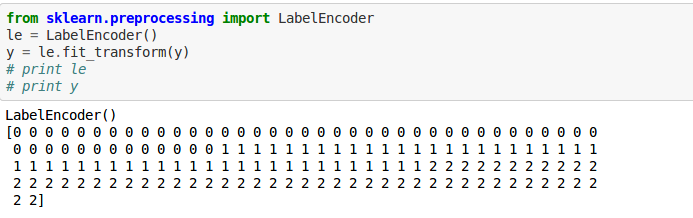
\includegraphics{label.png}


\end{document}

